\documentclass[conference]{IEEEtran}
\IEEEoverridecommandlockouts
% The preceding line is only needed to identify funding in the first footnote. If that is unneeded, please comment it out.
\usepackage{cite}
\usepackage{amsmath,amssymb,amsfonts}
\usepackage{algorithmic}
\usepackage{graphicx}
\usepackage{textcomp}
\usepackage{xcolor}
\def\BibTeX{{\rm B\kern-.05em{\sc i\kern-.025em b}\kern-.08em
    T\kern-.1667em\lower.7ex\hbox{E}\kern-.125emX}}
\begin{document}

\title{Paper Title*\\
{\footnotesize \textsuperscript{*}Note: Sub-titles are not captured in Xplore and
should not be used}
\thanks{Identify applicable funding agency here. If none, delete this.}
}

\author{\IEEEauthorblockN{1\textsuperscript{st} Carlos Enrique Tisza Vargas}
\IEEEauthorblockA{\textit{dept. name of organization (of Aff.)} \\
\textit{Ricardo Palma (of Aff.)}\\
Lima, Peru \\
ctiszav@gmail.com}

}

\maketitle

\begin{abstract}
el presente trabajo compila el resultado del estudio de 10 paper relacionados con los temas de clasificacion multilabel multimodal sobre publicaciones del portal ACM.
En la actualidad hay una busqueda de nuevos metodos o combinacion  de metodos existentes para mejorar los procesos de clasificacion de variables ,
Uno de los pilares sobre los cuales estan basados los paper es en incrementar el ratio de clasificacion utilizando muchas fuentes de datos.
\end{abstract}

\begin{IEEEkeywords}
component, formatting, style, styling, insert
\end{IEEEkeywords}

\section{Introduction}
En el mundo real generalmente la representación de objetos que se desean analizar se componen de multiples etiquetas y se pueden representar con multiples representaciones modales.

Por ejemplo los articulos suelen tener texto e imagenes otro ejemplo seria  de  el historial de datos de un usuario en forma de registros el cual se analiza con la finalidad de generar un perfil a este se le podria adicionar grabaciones de audios y videos con la finalidad de mejorar la predicción.

Los Sistemas de recomendación híbrido atacan el problema de analizar multiple fuentes de datos con multiple etiquetas
 

Procesar grandes cantidades de información y clasificarlas es un problema 

Debido a la cantidad de poder de calculo que se necesita para procesar enormes bases de datos, es por eso que es necesario desaroollar tecnicas para optimizar los procesos de clasificación. aun mas cuando los procesos requieren clasificaciones en tiempo real .

 


Se han realizado esfuerzos para mejorar la eficacia del aprendizaje multi-etiqueta con etiquetas incompletas. Actualmente la mayoria de técnicas para el  asumen que las características de los datos de entrada estan completas.

En el mundo real los datos con etiquetas incompletas son comunes y la co-ocurrencia de caracteristicas altamente incompletas y de asignaciones de etiquetas débiles es un desafío dado que los algoritmos de multietiqueta no son directamente aplicables.



\section{Sistemas de recomendación híbridos}

\subsection{Descripción del problema}

La tienda online ASOS atrajo 174 de millones de visitantes durante diciembre de 2017 y tiene 16 millomnes de clientes activos. En todo momento tiene 85K de productos activos y aproximadamente 5k de nuevos productos entran a la tienda cada semana. a traves de los anos diferentes divisiones de la compania producen y consumen diferentes atributos de los productos algunos no se muestran al cliente final por lo tanto no estan completos y no son consistentes.

En este trabajo se muestra como se ha realizado una caracterizacion de un cojunto de atributos de productos y como se habilita la personalizacion de la expereiencia de un cliente mostrandole lo mas relevante para el.


\begin{table}[]
\centering
\caption{Representación de los atributos de los productos}
\begin{tabular}{lllll}
producto & tipo  & segmento   & patron & ... \\
A        & dress & ?          & floral & ?   \\
B        & dress & girly girl & ?      & ... \\
C        & skirt & ?          & check  & ?   \\
...      & ...   & ...        & ...  & ...    
\end{tabular}

\end{table}

\subsection{Diseño}

\subsubsection{Clasificación de imagenes}
La moda es un dominio muy visual y con la popularidad del aprendizaje profundo ya existe en la literatura bastantes enfoques para clasificar y predecir los atributos de ropa a partir de la imagen. para este caso se aplicó la red neuronal convolucional VGG16 con datos entrenados de ImageNet

\subsubsection{Clasificación de Texto}
Las redes neuronales convolucionales han demostrado tambien ser efectivas en clasificar no solo imágenes sino también
texto. Las oraciones se pueden tratar como secuencias de palabras, donde
Cada palabra a su vez puede representarse como un vector en un \textit{multidimensional
word embedding space}.

\subsubsection{Multi-modal Fusion}

Cada modelidad es procesada en diferentes redes, despues de llegar a un nivel las resultados son concatenados siguiendo capas multimodales , la politica de la red esta aprendiendo a decidir que clasificador utilizara.

En la figura 1\cite{b1} se muestra la arquitectura de una red de fusión multi-modal.




\begin{figure*}
  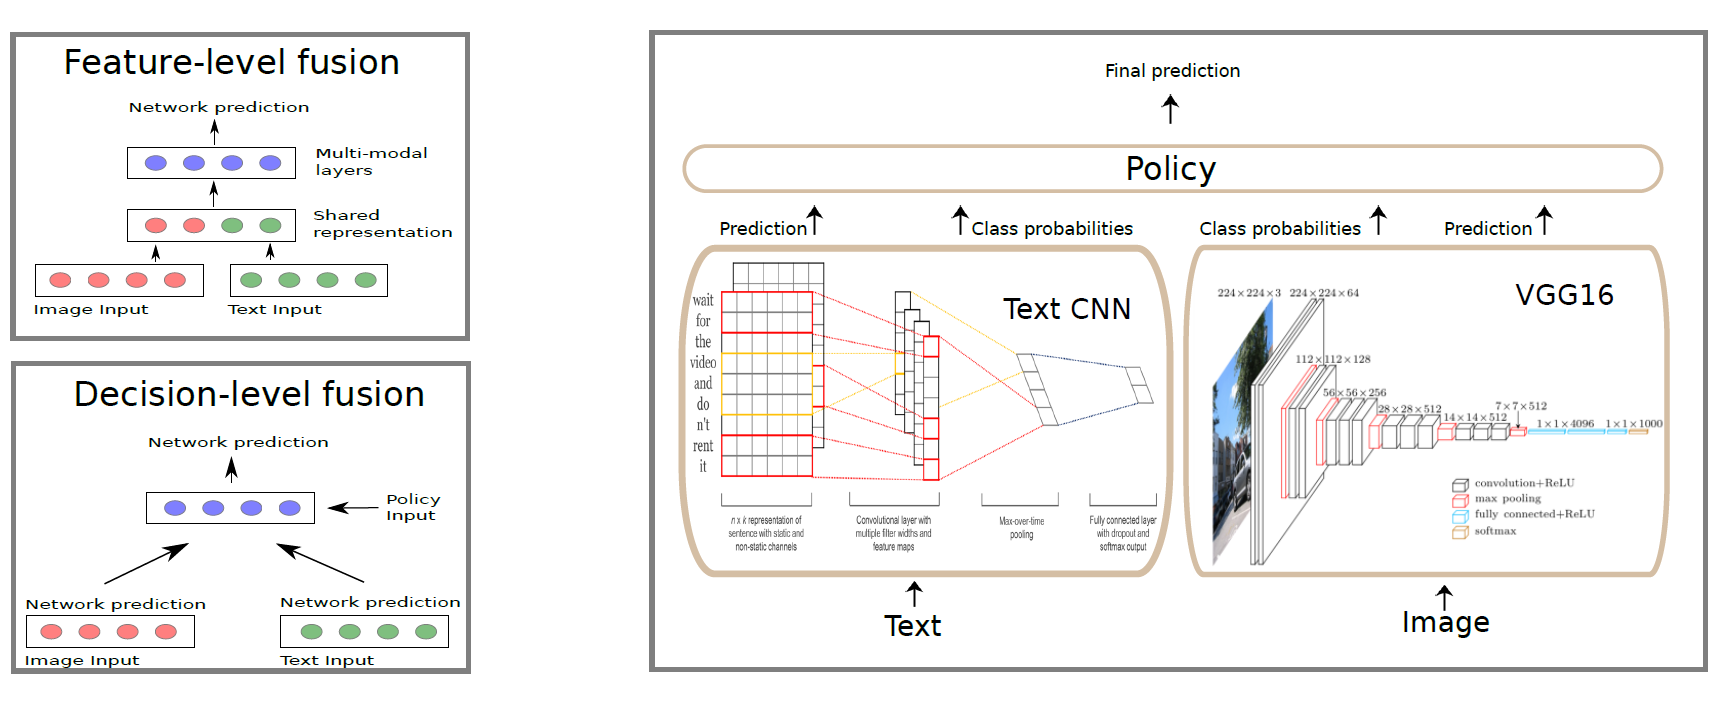
\includegraphics[width=\textwidth,height=4cm]{figura1.png}
  \caption{Multimodal Fusión}
  \label{fig}
\end{figure*}


\subsubsection{Multi-Task learning with Missing Labels}
Los datos de entrenamiento requerirían implementar una función de pérdida personalizada o enmascarar capas para evitar propagar errores cuando una etiqueta no está disponible.

Se implementó la arquitectura mostrada en la figura 4, aquí los cuadros de color gris representan las entradas a la red  , entre parentesis se muestran el tamaño de la salida de cada red , en azul las capas ocultas y rojo las capas de salidad .  

en la practica como se ilustra en la figura se contruye un modelo para cada atributo pero todos comparten los mismos parámetros hasta laa capa de salida. Tambien se prepapa un conjunto de datos para cada atributo , los cuales son actualizados mediante el enjoque de descenso de gradiente(SGD) durante el entrenamiento . 
\begin{figure}
\centerline{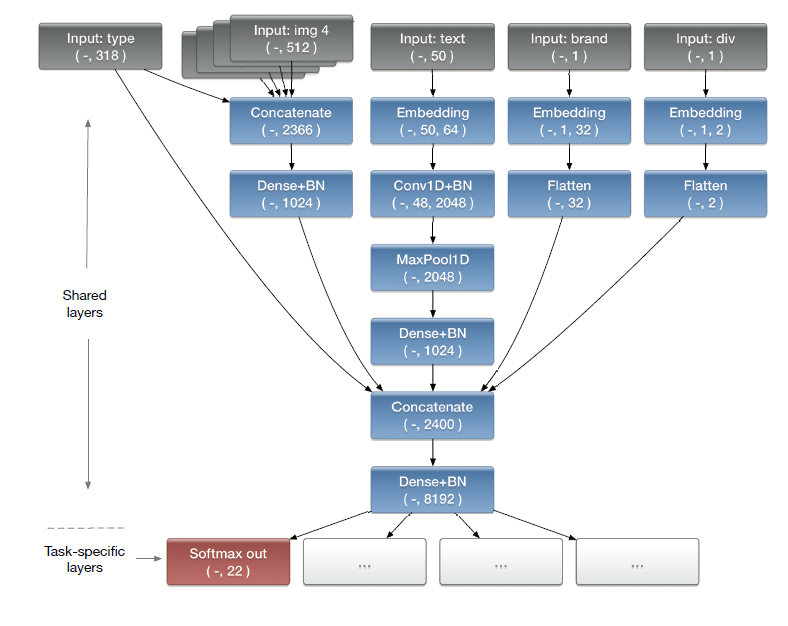
\includegraphics[width=\textwidth,width=9cm]{figura4.png}}
\caption{Multi-modal multi-task architecture}
\label{fig}
\end{figure}

\subsection{Resultados}


La tabla 2 muestra los resultados de los experimentos de recomendanciones , promedios y desviaciones estandares despues de 10 ejecuciones . Se observa que el modelo hibrido es el mas efectivo comparado con otros enfoques como filtrado colaborativo .



\begin{table}[]
\centering
\caption{Resultados}
\begin{tabular}{lllll}
		 & prec@10  & recall@10\\
Popularity        & 0.00231 & 0.00765\\
Collaborative        & 0.00277±0.00011& 0.00931±0.00036 \\
Content        & 0.00246±0.00011 & 0.00755±0.00191\\
Hybrid    & 0.00313±0.00015   & 0.00960±0.00252 
\end{tabular}
\end{table}

\section{A Multi-Modal Multi-Instance
Multi-Label Deep Network with Optimal Transport}



Este trabajo el objetivo es predecir y explorar la correlacción de las etiquetas  simultaneamente. se propuso usar la red M3DN (modelo Multi-modal Multi-instancia Multietiqueta) que modela las redes independientes para cada modalidad e impone la  consitencia en el bag level que se utiliza para la predicción de diferentes modalidades que tienen etiquetas correlacionadas

Se denomina bag a cada muestra la cual esta representada por varias instancias  

Se tiene N bags los cuales pueden ser positivos o negativos , además cada bag tiene k modalidades las cuales tienen un conjunto de instancias que son los datos de entrenamiento.


\subsection{Transporte óptimo} 
el transporte optimo se define como la distancia minima que existe entre dos distribuciones.

\subsection{Multi-Modal Multi-instance Multi-label Deep Network (M3DN)}
En la figura 3 se muestra las dos modalidades , el bag de 4 imagenes y el bag de 5 parrafos de texto.
En base a la teoria del transporte optimo, M3DN adopta la distancia ooptima de transporte para medir la ccalidad de la prediccion que captura la informacion geolmetrica del esllpacio de la etiqueta subyacente  .

ademas M3DN automaticamente aoprende de la correlacion entre las etiquetas de las diferentes modalidades. M3DN automaticamente aprenden los predictores de las diferentes modalidades .

\begin{figure*}
  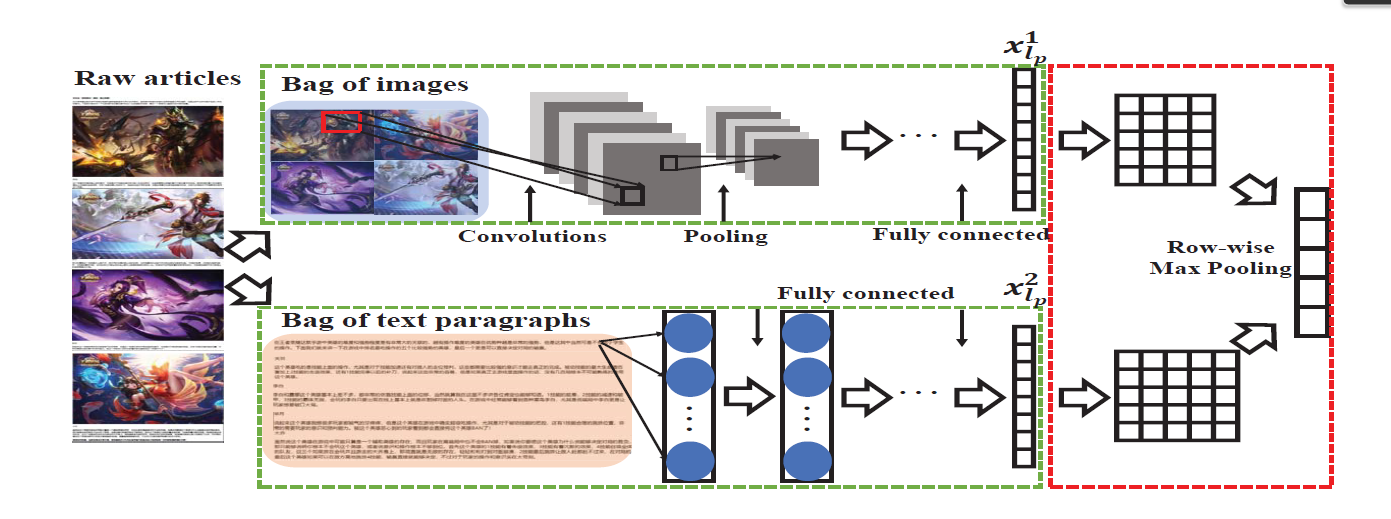
\includegraphics[width=\textwidth,height=4cm]{figura2.png}
  \caption{Multimodal Fusión}
  \label{fig}
\end{figure*}


\subsection{Resutados}

Comparación de los resultados (mean+std) de M3DM sobre los datos de WKG Game-Hub.

 \begin{figure*}
  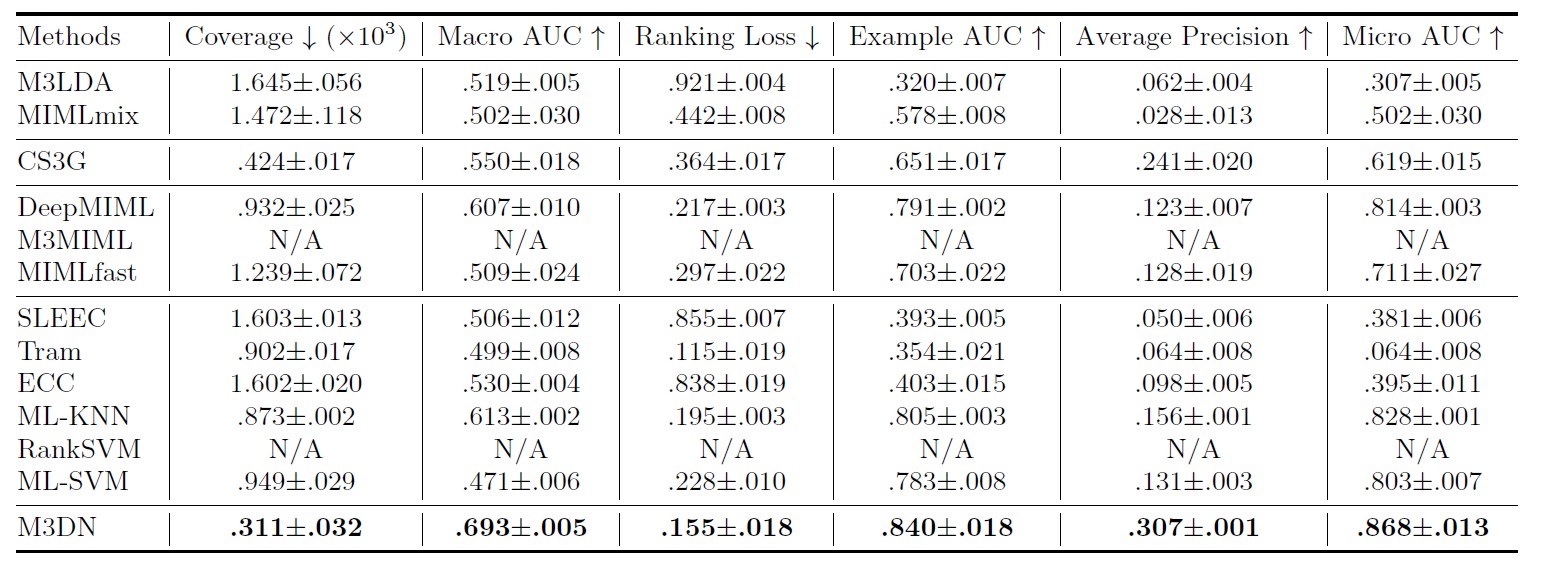
\includegraphics[width=\textwidth,height=4cm]{figura5.png}
  \caption{Resultados}
  \label{fig}
\end{figure*}

\subsection{Exploración de Correlación de etiquetas}

Teniendo en cuenta que M3DN puede aprender la correlación de la etiqueta explícitamente.
En esta subsección, examinamos la efectividad de M3DN.

La exploración se lleva a cabo en el conjunto de datos  real de
WKG Game-Hug. Muestreamos aleatoriamente 27 etiquetas, y
la métrica del terreno aprendida por M3DN se muestra en la Figura 4, y
escalamos el valor original en la matriz de costos en [-1, 1]. rojo
color indica una correlación positiva, y azul indica una correlación negativa.
\begin{figure}
\centerline{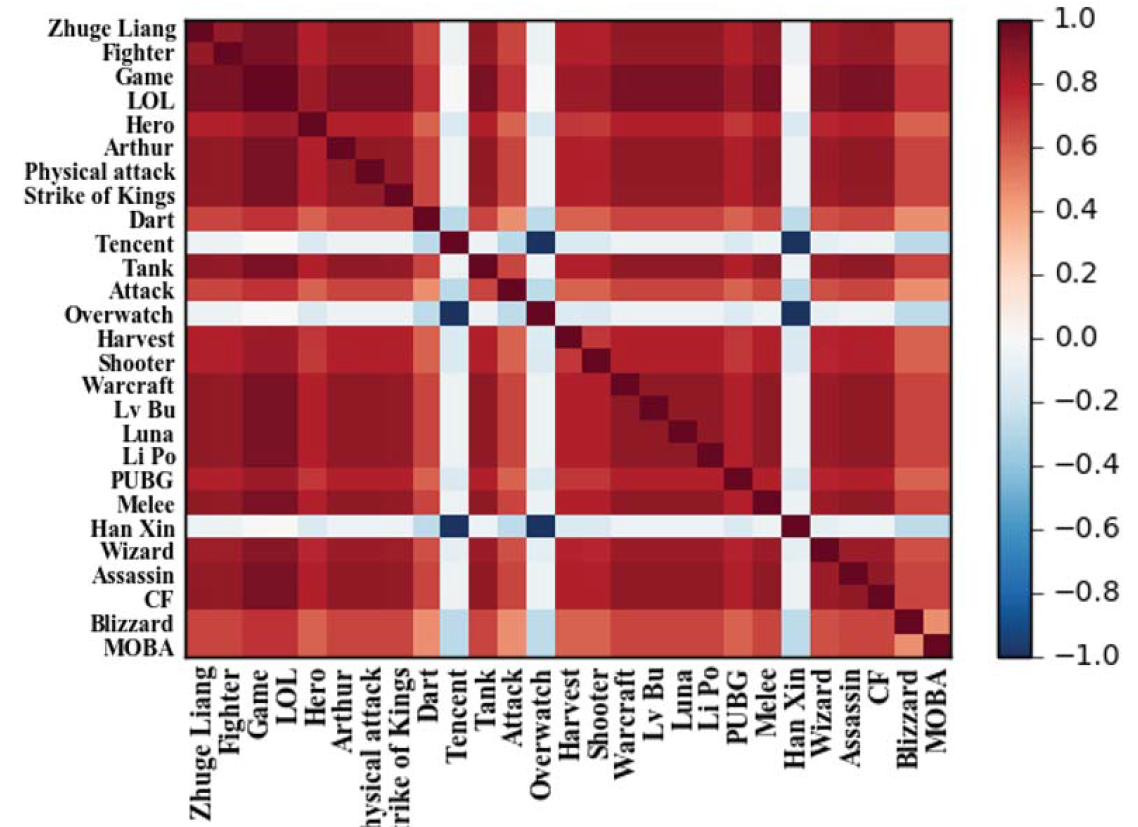
\includegraphics[width=\textwidth,width=9cm]{figura6.png}}
\caption{Multi-modal multi-task architecture}
\label{fig}
\end{figure}

\section{Multimodal Sentiment Analysis To Explore the Structureof Emotions}


Se utiliza un enfoque para el análisis de sentimientos multimodal usando redes neuronales profundas combinando el análisis visual y el procesamiento de lenguaje natural. el objetivp a diferencia de de otras redes donde el objetivo es predecir si unaa sentencia es positivo o negaativo aqui se el objetivo es inferir el estado emocional latente del usuario. Por lo tanto, nos centramos en predecir las etiquetas de palabras de emoción unidas por los usuarios a sus publicaciones de Tumblr, tratando estas "emociones autoinformadas". Demostramos que nuestro modelo multimodal que combina las características  , automáticamente ofrece listas de palabras sensibles asociadas con las emociones. Exploramos la estructura de emociones que implica nuestro modelo y la comparamos con lo que se ha publicado en la literatura de psicología, y validamos nuestro modelo en un conjunto de imágenes que se han utilizado en estudios de psicología. Por último, nuestro trabajo ofrece una herramienta para el auge del estudio académico de imágenes, tanto de fotografías como de mimos, en redes sociales.


\section{La base de datos Tumblr}


Tumblr es un servicio de microblogging donde los usuarios publican contenido multimedia  que a menudo contiene los siguientes atributos: una imagen, texto,
y etiquetas. El enfoque es que a partir de métodos de análisis de sentimientos centrados  puramente en una clasificación de positivo y negativos se usan las etiquetas de palabras de emoción como las etiquetas que deseamos predecir. Al considerar estas etiquetas de palabras como indicadores de emoción que esta asociado al estado mental del usuario al escribir una publicación, podemos usarlos como un proxy para la emoción autoinformada, y
por lo tanto, un proxy para el estado emocional subyacente del usuario.
Para construir nuestro conjunto de datos, se realizaron consultas a través del api de Tumblr buscando las  emociones que van apareciendo en las etiquetas. Las 15 emociones
retenidas fueron aquellos con altas frecuencias relativas en Tumblr.

\begin{figure}
\centerline{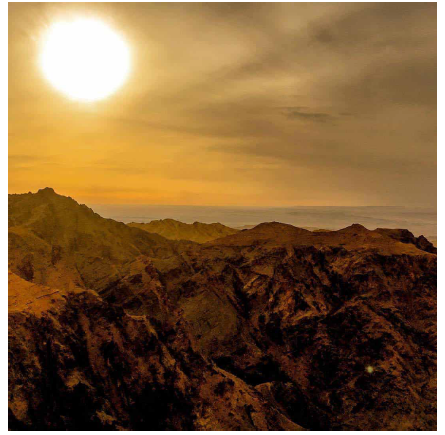
\includegraphics[width=\textwidth,width=9cm]{figura8.png}}
\caption{Optimistic: "Recuerda que nada importa, como te puedes sentir triste o mal cuando el sol esta por salir"}
\label{fig}
\end{figure}

\begin{figure}
\centerline{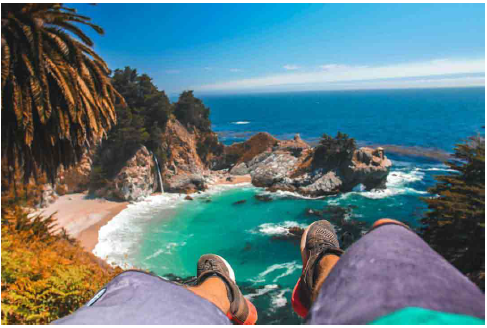
\includegraphics[width=\textwidth,width=9cm]{figura9.png}}
\caption{Relajado: Me encuentro ralajado con la vista impresionante}
\label{fig}
\end{figure}

\subsection{Deep Sentiment: la red neuronal multinodos}
Por un lado, la imagen de entrada, redimensionada a (224,224,3) se introduce en el Inicio
red y produce un vector de tamaño 256. Por otro lado, el texto se proyecta en un espacio de alta dimensión. que posteriormente pasa por una capa LSTM con 1024
unidades. Las dos modalidades se concatenan y se introducen en
Una capa densa. La capa de salida de softmax final da la probabilidad
Distribución sobre el estado emocional del uso.
\begin{figure}
\centerline{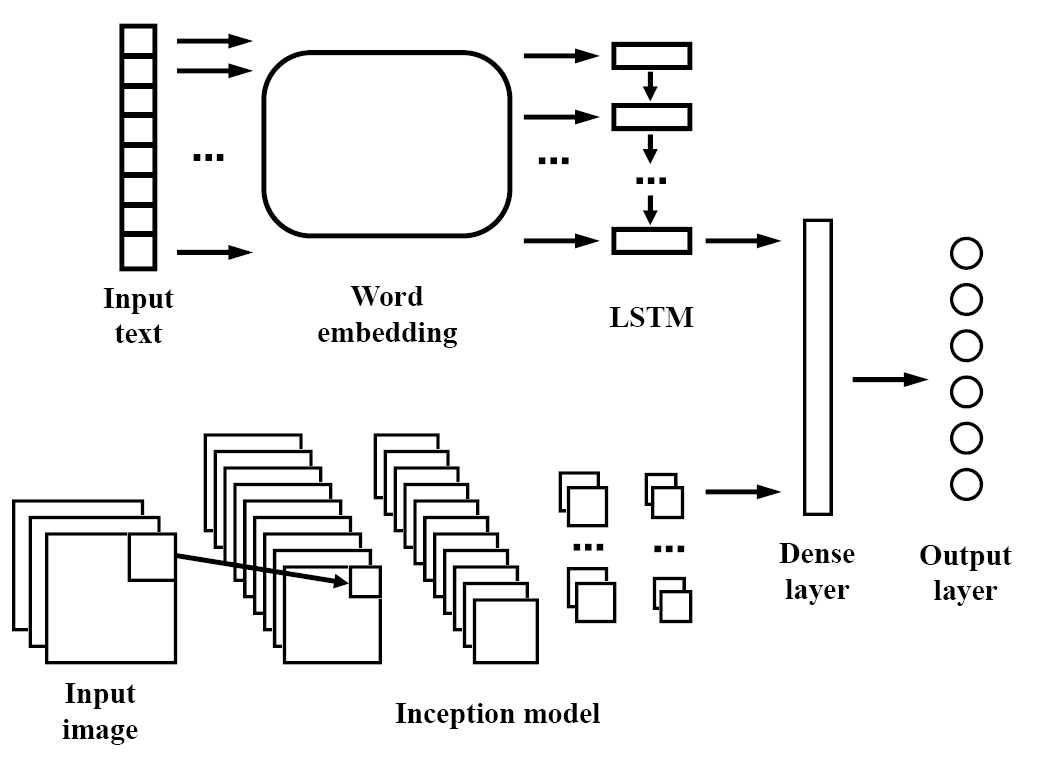
\includegraphics[width=\textwidth,width=9cm]{figura7.png}}
\caption{Relajado: Me encuentro ralajado con la vista impresionante}
\label{fig}
\end{figure}

\subsection{Resultados}
Usando texto solo, la precisión de la prueba es del 69%, casi el doble del
La precisión del modelo de imagen, esto sugiere que en Tumblr, el texto es un
mejor predictor de la emoción que las imágenes, como ilustramos en la fig 9 y 10
al combinar texto e imágenes, Deep Sentiment logra un 80% de precisión con la data de  entrenamiento y 72% de precisión con los datos de prueba, superando significativamente a los modelos de solo imagen y ligeramente superior al modelo de solo texto
\begin{figure}
\centerline{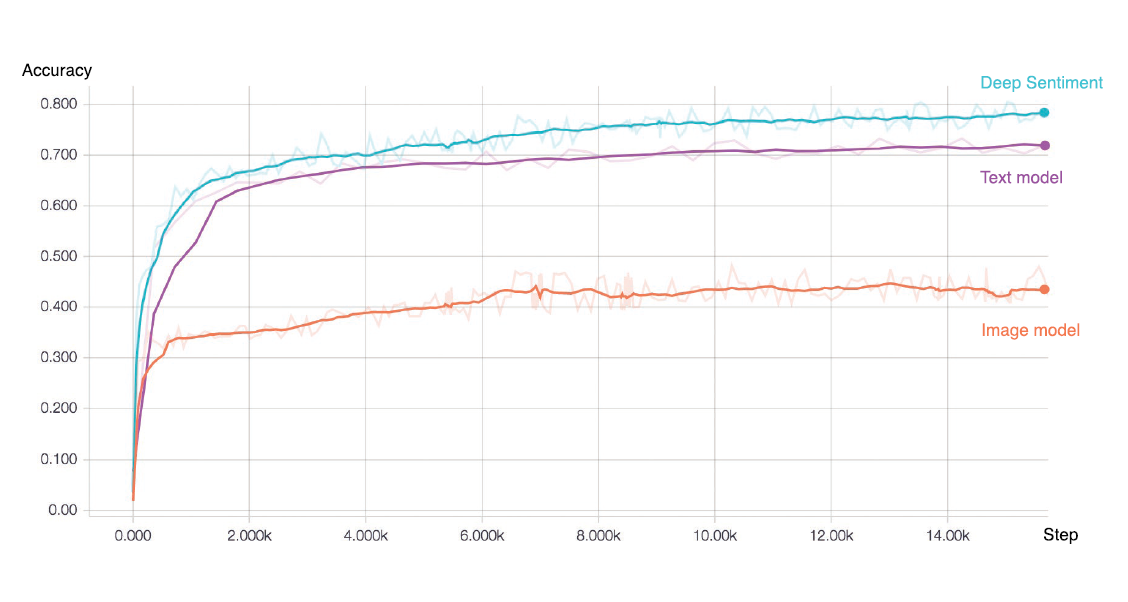
\includegraphics[width=\textwidth,width=9cm]{figura10.png}}
\caption{Precisión con la data de entrenamiento}
\label{fig}
\end{figure}

\begin{figure}
\centerline{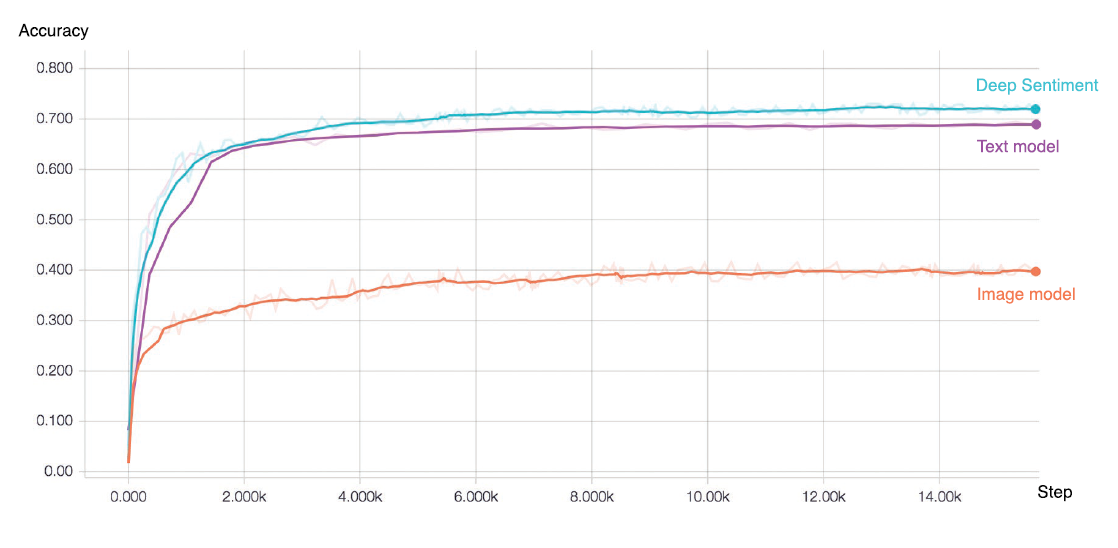
\includegraphics[width=\textwidth,width=9cm]{figura11.png}}
\caption{Precisión con la data de prueba}
\label{fig}
\end{figure}

\subsection{Multi-label Learning with Highly Incomplete Data via Collaborative Embedding}

Se han dedicado enormes esfuerzos a mejorar la eficacia del aprendizaje multi-etiqueta con asignaciones de etiqueta incompletas. La mayoría de las técnicas actuales asumen que las características de entrada de las instancias de datos están completas. Sin embargo, la co-ocurrencia de características altamente incompletas y asignaciones de etiquetas débiles es un desafío y un problema ampliamente percibido en el aprendizaje de etiquetas múltiples del mundo real solicitudes debido a una serie de razones prácticas, incluyendo recopilación incompleta de datos, etiquetas moderadas de anotadores, etc.
Los algoritmos de aprendizaje de etiquetas múltiples existentes no son directamente aplicables cuando las características observadas son altamente incompletas. En este se ataca este problema proponiendo una multi-etiqueta débilmente supervisada
Enfoque de aprendizaje, basado en la idea de incrustación colaborativa.
Este enfoque proporciona un marco flexible para llevar a cabo eficientemente la clasificación de etiquetas múltiples en modo transductor e inductivo
mediante el acoplamiento del proceso de reconstrucción de características faltantes y asignaciones de etiquetas débiles en un marco de optimización conjunta. Es diseñado para recuperar colaborativamente información de características y etiquetas, y extraer la asociación predictiva entre el perfil de la característicay la etiqueta  multi-etiqueta de la misma instancia de datos.


\begin{figure}
\centerline{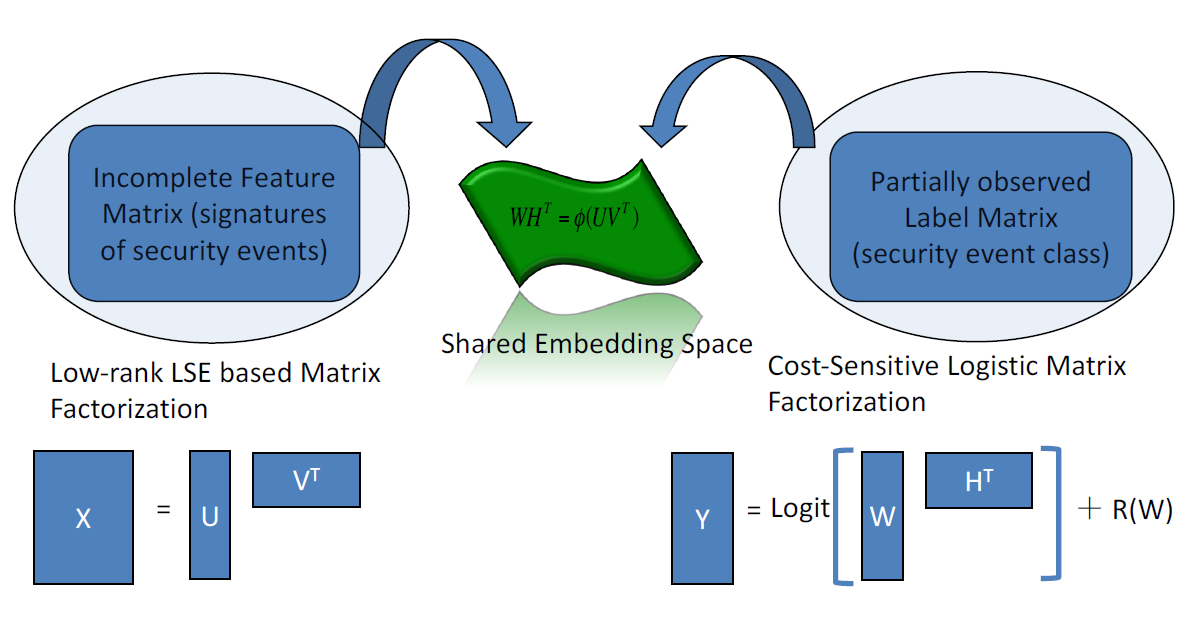
\includegraphics[width=\textwidth,width=9cm]{figura12.png}}
\caption{Collaborative Embedding: A Transfer Learning Approach}
\label{fig}
\end{figure}

\begin{figure}
\centerline{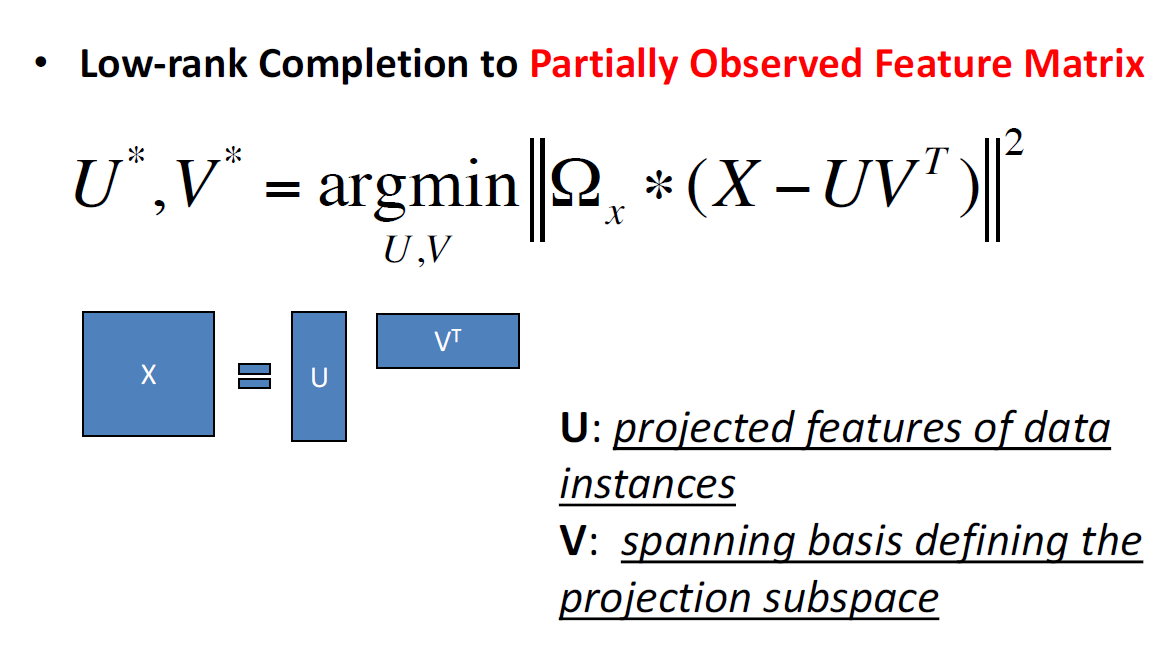
\includegraphics[width=\textwidth,width=9cm]{figura13.png}}
\caption{Feature Matrix Completion}
\label{fig}
\end{figure}

\begin{figure}
\centerline{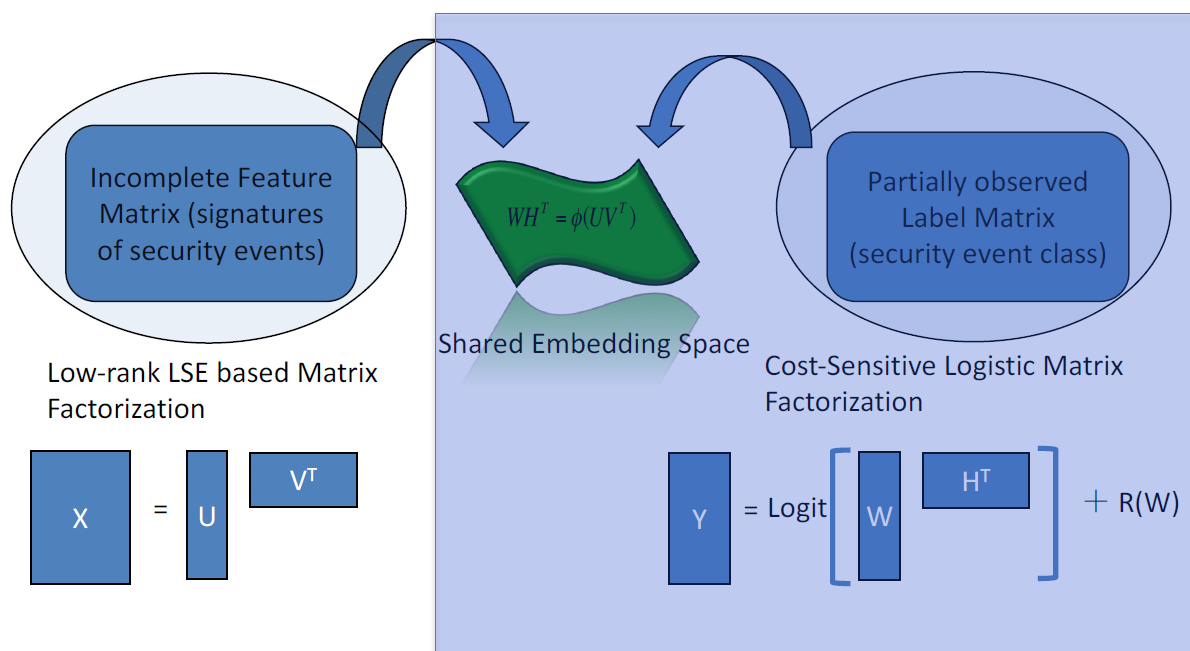
\includegraphics[width=\textwidth,width=9cm]{figura14.png}}
\caption{Collaborative Embedding: A Transfer Learning Approach}
\label{fig}
\end{figure}


\begin{figure}
\centerline{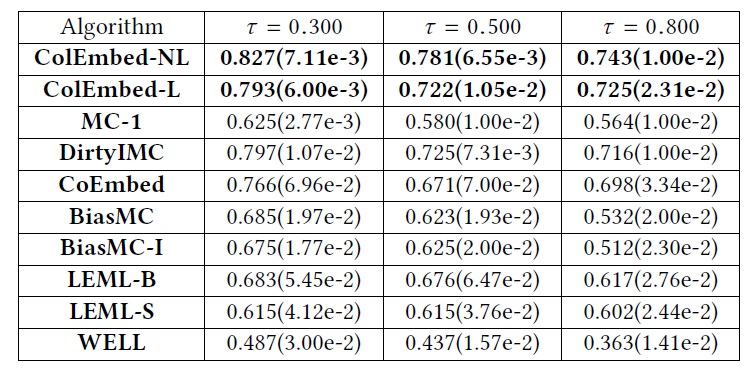
\includegraphics[width=\textwidth,width=9cm]{figura15.png}}
\caption{Mean (standard deviation) of transductive Macro-
AUC of all involved algorithms on EventCat}
\label{fig}
\end{figure}

\begin{figure}
\centerline{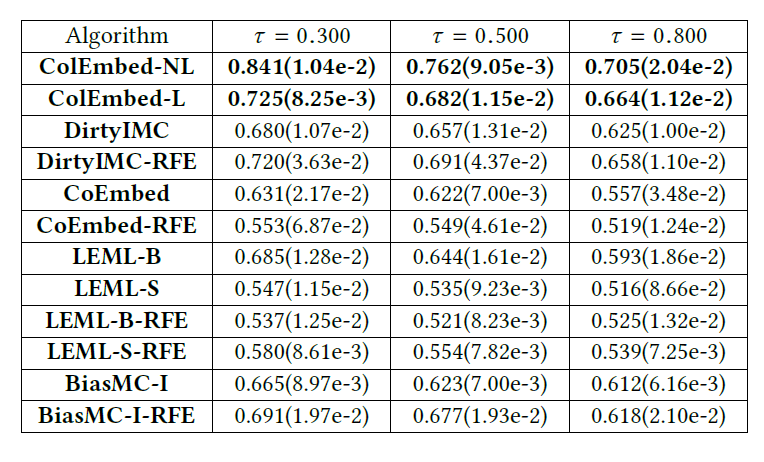
\includegraphics[width=\textwidth,width=9cm]{figura16.png}}
\caption {(standard deviation) of inductive Macro-AUC of all involved algorithms on EventCat}
\label{fig}
\end{figure}


\subsection{AnnexML:ApproximateNearestNeighborSearch forExtremeMulti-labelClassification }

Los métodos de clasificación de etiquetas múltiples extremas se han utilizado ampliamente en tareas de clasificación a escala web, como el etiquetado de páginas web y la recomendación de productos. En este documento se presentamos un método novedoso de incrustación de gráficos llamado "AnnexML". En la etapa de entrenamiento, AnnexML construye un gráfico de vectores de etiqueta para el vecino más cercano al k e intenta reproducir la estructura del gráfico en el espacio de incrustación.
La predicción se realiza de manera eficiente mediante el uso de un aproximado
método de búsqueda de vecino más cercano que explora de manera eficiente el gráfico de vecino k más cercano aprendido en el espacio de incrustación. Se realizaron evaluaciones en varios conjuntos de datos de gran escala en el mundo real y se comparo el método con los últimos métodos de vanguardia. Los resultados experimentales muestran que nuestro AnnexML puede mejorar significativamente la precisión de la predicción, especialmente en conjuntos de datos que tienen un espacio de etiqueta más grande. Además, AnnexML mejora la compensación entre el tiempo de predicción y la precisión. Al mismo nivel de precisión, el tiempo de predicción de AnnexML fue hasta 58 veces más rápido que el de SLEEC, que es un método basado en la incorporación de tecnología de punta.



\section*{Acknowledgment}


\section*{References}

Please number citations consecutively within brackets \cite{b1}. The 
sentence punctuation follows the bracket \cite{b2}. Refer simply to the reference 
number, as in \cite{b3}---do not use ``Ref. \cite{b3}'' or ``reference \cite{b3}'' except at 
the beginning of a sentence: ``Reference \cite{b3} was the first $\ldots$''

Number footnotes separately in superscripts. Place the actual footnote at 
the bottom of the column in which it was cited. Do not put footnotes in the 
abstract or reference list. Use letters for table footnotes.

Unless there are six authors or more give all authors' names; do not use 
``et al.''. Papers that have not been published, even if they have been 
submitted for publication, should be cited as ``unpublished'' \cite{b4}. Papers 
that have been accepted for publication should be cited as ``in press'' \cite{b5}. 
Capitalize only the first word in a paper title, except for proper nouns and 
element symbols.

For papers published in translation journals, please give the English 
citation first, followed by the original foreign-language citation \cite{b6}.

\begin{thebibliography}{00}
\bibitem{b1} Tom Zahavy, Alessandro Magnani, Abhinandan Krishnan, and Shie Mannor. 2016.
Is a picture worth a thousand words? A Deep Multi-Modal Fusion Architecture
for Product Classification in e-commerce. arXiv preprint arXiv:1611.09534 (2016).
\bibitem{b2} J. Clerk Maxwell, A Treatise on Electricity and Magnetism, 3rd ed., vol. 2. Oxford: Clarendon, 1892, pp.68--73.
\bibitem{b3} I. S. Jacobs and C. P. Bean, ``Fine particles, thin films and exchange anisotropy,'' in Magnetism, vol. III, G. T. Rado and H. Suhl, Eds. New York: Academic, 1963, pp. 271--350.
\bibitem{b4} K. Elissa, ``Title of paper if known,'' unpublished.
\bibitem{b5} R. Nicole, ``Title of paper with only first word capitalized,'' J. Name Stand. Abbrev., in press.
\bibitem{b6} Y. Yorozu, M. Hirano, K. Oka, and Y. Tagawa, ``Electron spectroscopy studies on magneto-optical media and plastic substrate interface,'' IEEE Transl. J. Magn. Japan, vol. 2, pp. 740--741, August 1987 [Digests 9th Annual Conf. Magnetics Japan, p. 301, 1982].
\bibitem{b7} M. Young, The Technical Writer's Handbook. Mill Valley, CA: University Science, 1989.
\end{thebibliography}



\end{document}
